\chapter{Interpretación y Resultados}
\label{ch:results}

En el presente capítulo se presentarán a detalle los resultados obtenidos por cada uno de los modelos propuestos para el pronóstico de demanda y el módelo para la maximización de ingresos. También se discutirá la forma en la que se deberán interpretar los resultados de los mismos y así evitar sacar conclusiones erróneas o fuera de contexto.

\section*{Interpretación de los modelos de pronóstico de ocupación}
Como hemos mencionado en capítulos anteriores, la solución propuesta se compone de dos modulos principales, el primero de ellos se encarga de pronosticar la demanda de cuartos noche, mientras que el segundo modulo toma esa información y calcula los precios por habitación  que  maximizan  el  ingreso  de  la  propiedad  tomando  en  cuenta  las restricciones definidas para la propiedad. A continuación explicaremos detalladamente los resultados obtenidos en cada uno de los modelos propuestos.


\subsection*{Modelo de regresión lineal generalizada con liga Poisson}

Este modelo toma como entrada las curvas de \emph{pickup} para una propiedad en específico, información de su ocupación histórica, lineas de tiempo de tarifa promedio, lineas de tiempo de tarifas publicas propias y de la competencia, etc. Al finalizar el procesamiento de la información se obtiene una matriz que contiene, entre otras variables, el parámetro $\beta_0$ y $\beta_1$ con el que se puede reconstruír la curva de pickup para un día futuro. De esta manera podemos obtener una buena aproximación de los cuartos que serán vendidos en cierto día y con qué velocidad se realizará esta venta.

A continuación se presenta un extracto de los resultados obtenidos por el modelo de pronóstico de demanda:

\begin{table}[H]
\begin{tabular}{lllllllllllll}
Hotel  & Dia         & AABeta0  & AAbeta1      & pred.beta0 & pred.beta1  \\
Hotel1 & 2018-01-01  & 2.335294 & -2.48986e-06 & 3.1595     & -0.1227     \\
Hotel1 & 2018-01-02  & 2.984073 & -2.81809e-06 & 3.9160     & -0.1160     \\
Hotel1 & 2018-01-03  & 3.301841 & -3.53557e-06 & 3.8740     & -0.1089     \\
Hotel1 & 2018-01-04  & 3.782523 & -2.29568e-06 & 4.1597     & -0.1028     \\
Hotel1 & 2018-01-05 & 3.761697 & -1.08967e-06 & 3.6982     & -0.0846    
\end{tabular}
\caption{Resultados arrojados por el modelo de predicción de demanda} 
\end{table}

Para poder reconstruír la curva de \emph{pickup} pronosticada se debe tomar los parámetros \emph{pred.beta0} y \emph{pred.beta1} para evaluar la siguiente expresión: $$E[y|x]=e^{\beta_0 + \beta_1x}$$

Dónde:
\begin{itemize}[noitemsep]
\item $E[y|x]$ = El valor esperado de cuartos noches para un día en específico dado $x$ días de antelación
\item $\beta_0$ = pred.beta0
\item $\beta_1$ = pred.beta1
\item $x$ = días de antelación
\end{itemize}

Para construír las curvas de \emph{pickup} pronósticadas se elige un día de la tabla de resultados arrojados por el modelo. Tomaremos los valores de \texttt{pred.beta0} y \texttt{pred.beta1} para el día elegido. Posteriormente x tomará valores de -1 a 25 para representar la curva en un rango de -1 a 25 días de antelación, siendo -1 las llegadas que llegan a la propiedad después de las 23:59 pm del día elegido.

Si tomamos el día 2018-01-04 tendríamos una tabla de interpretación como la que se muestra a continuación:

$$pred.beta0 = 4.1597$$ $$pred.beta1 = -0.1028$$

\begin{table}[H]
\centering
\begin{tabular}{cc}
Antelación & Cuartos Ocupados (Predicción) \\
-1         & 71                            \\
0          & 64                            \\
1          & 58                            \\
2          & 52                            \\
3          & 47                            \\
4          & 42                            \\
5          & 38                            \\
6          & 35                            \\
7          & 31                            \\
8          & 28                            \\
9          & 25                            \\
10         & 23                            \\
11         & 21                            \\
12         & 19                            \\
13         & 17                            \\
14         & 15                            \\
15         & 14                            \\
16         & 12                            \\
17         & 11                            \\
18         & 10                            \\
19         & 9                             \\
20         & 8                             \\
21         & 7                             \\
22         & 7                             \\
23         & 6                             \\
24         & 5                             \\
25         & 5                            
\end{tabular}
\caption{Interpretación de resultados arrojados por el modelo de pronóstico de demanda}
\end{table}

Podemos ver que en esta expresión \texttt{pred.beta0} indica cuantos cuartos ocupados se tendrán para el día estudiado, mientras que \texttt{pred.beta1} dicta cuantos cuartos incrementan conforme X se acerca a 0 (día de la llegada de los huéspedes al hotel).

Evaluando esta expresión en distintas fechas obtenemos las siguientes curvas de pronóstico de ocupación:

\begin{figure}[H]
  \centering
      \includegraphics[width=\maxwidth,height=10cm]{figures/Resultados-1}  
  \caption{Curva de pickup real vs pronosticada (1)}
\end{figure}

\begin{figure}[H]
  \centering
      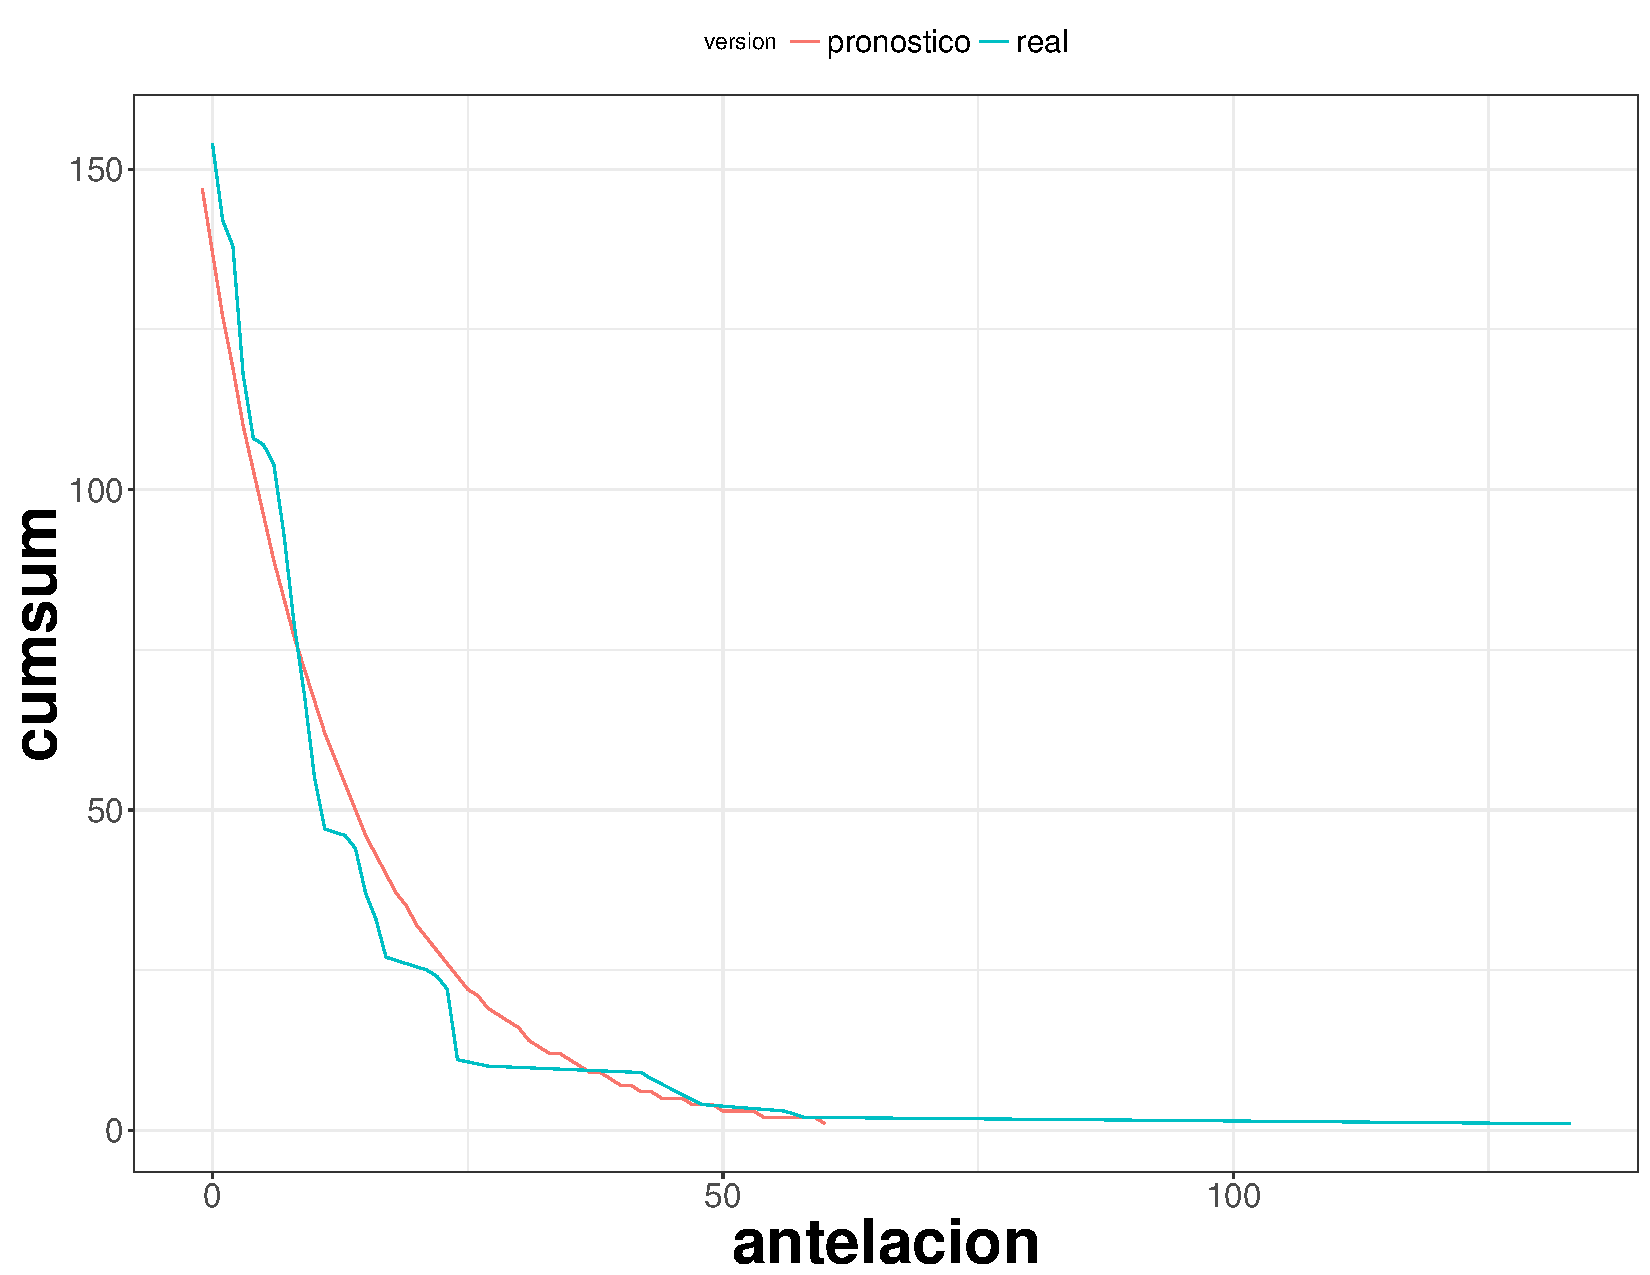
\includegraphics[width=\maxwidth,height=8cm]{figures/Resultados-2}  
  \caption{Curva de pickup real vs pronosticada (2)}
\end{figure}

\begin{figure}[H]
  \centering
      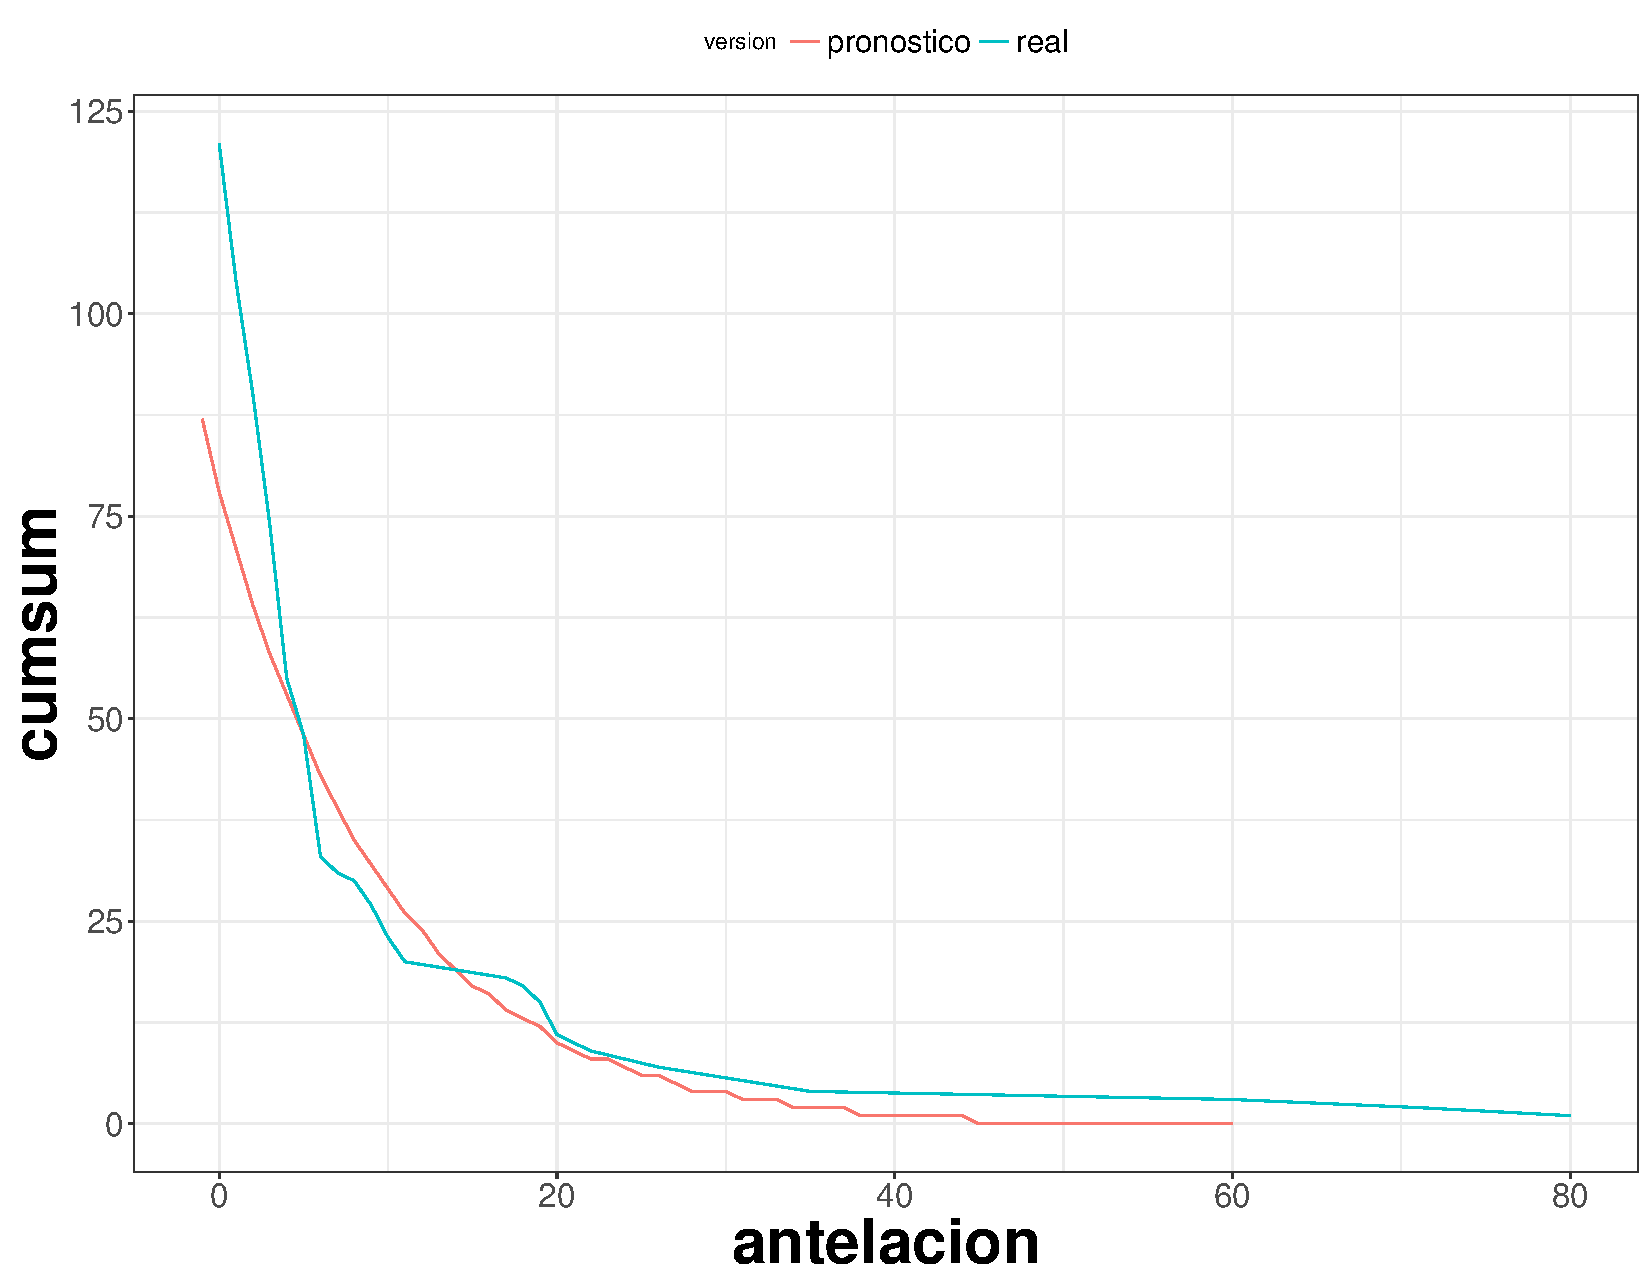
\includegraphics[width=\maxwidth,height=8cm]{figures/Resultados-3}  
  \caption{Curva de pickup real vs pronosticada (3)}
\end{figure}

\begin{figure}[H]
  \centering
      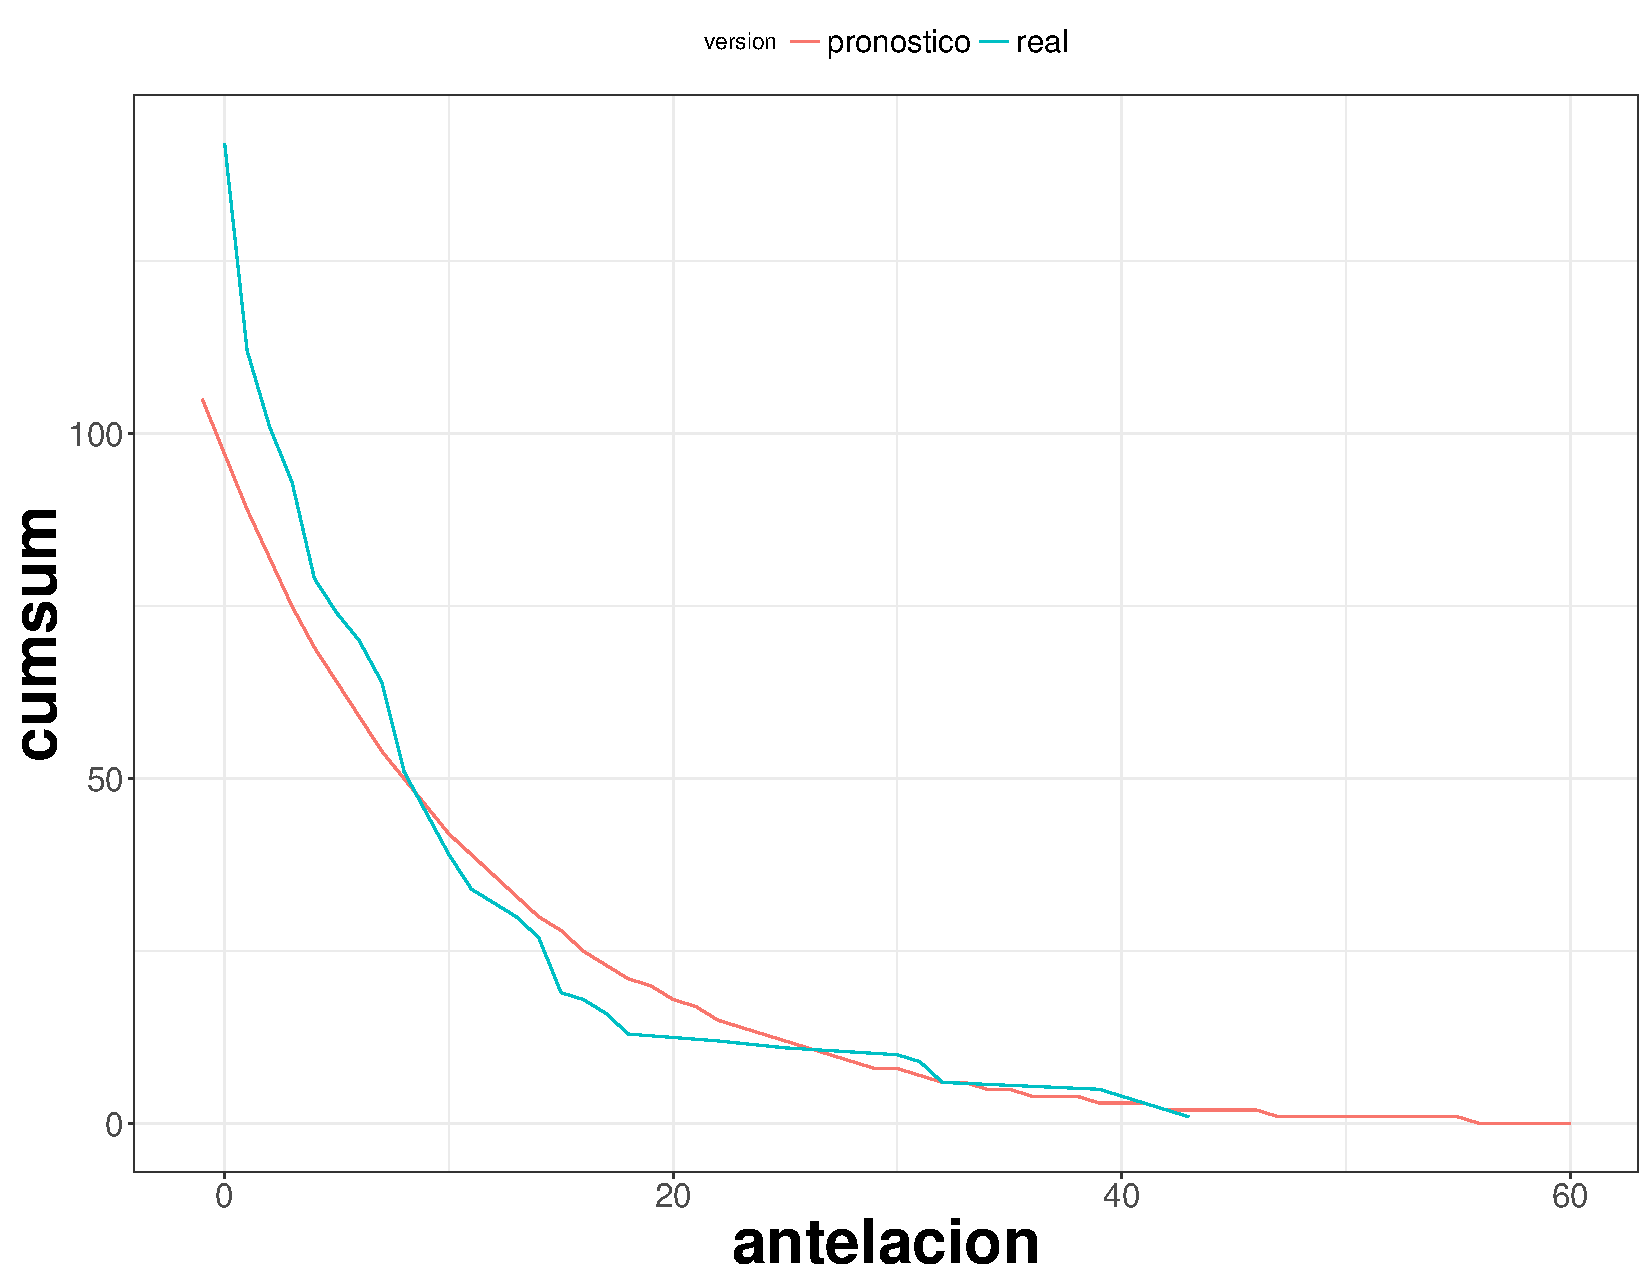
\includegraphics[width=\maxwidth,height=10cm]{figures/Resultados-4}  
  \caption{Curva de pickup real vs pronosticada (4)}
\end{figure}

Podemos observar que la curva pronosticada tiene un buen ajuste sobre la curva real en la mayoría de los casos.

Para realizar la validación del modelo se dividió el data set en dos partes, la primera parte se utilizó para el entrenamiento del modelo y la segunda parte para la validación del mismo, de esta forma se pudo comparar el pronóstico de demanda arrojado por el modelo contra la demanda real de la propiedad en 220 días para el año 2018.

Para evaluar el desempeño del modelo se utilizó la medida \emph{MAPE} definida como: $$MAPE=\frac{1}{n}\sum_{t=1}^{n}|\frac{y_t-h_t}{y_t}|$$

Dónde:
\begin{itemize}[noitemsep]
  \item n = Número de puntos ajustados
  \item $y_t$ = Cuartos noche vendidos en el tiempo $t$
  \item $h_t$ = Venta de cuartos noche pronósticada en el tiempo $t$
\end{itemize}


El \emph{MAPE} observado durante la validación del modelo fue de 17.67\%.

\subsection*{Modelo de regresión de Ridge}

Durante la implementación del modelo basado en una regresión de Ridge, se utilizaron varios valores para el parámetro $\alpha$ (factor de regularización). De los resultados que obtuvimos notamos que el modelo tuvo un mejor desempeño cuando $\alpha = 1*e^{-15}$. El parámetro $\alpha$ también es conocido como el \emph{coeficiente de regularización}, el cual es usado para mejorar el condicionamiento del problema y reduce la varianza de las predicciones generadas. Mientras más grande es $\alpha$ mayor es la regularización. 

En la siguiente gráfica se muestra el efecto que tiene los distintos valores de $\alpha$ sobre las predicciones generadas:

\begin{figure}[H]
  \centering
      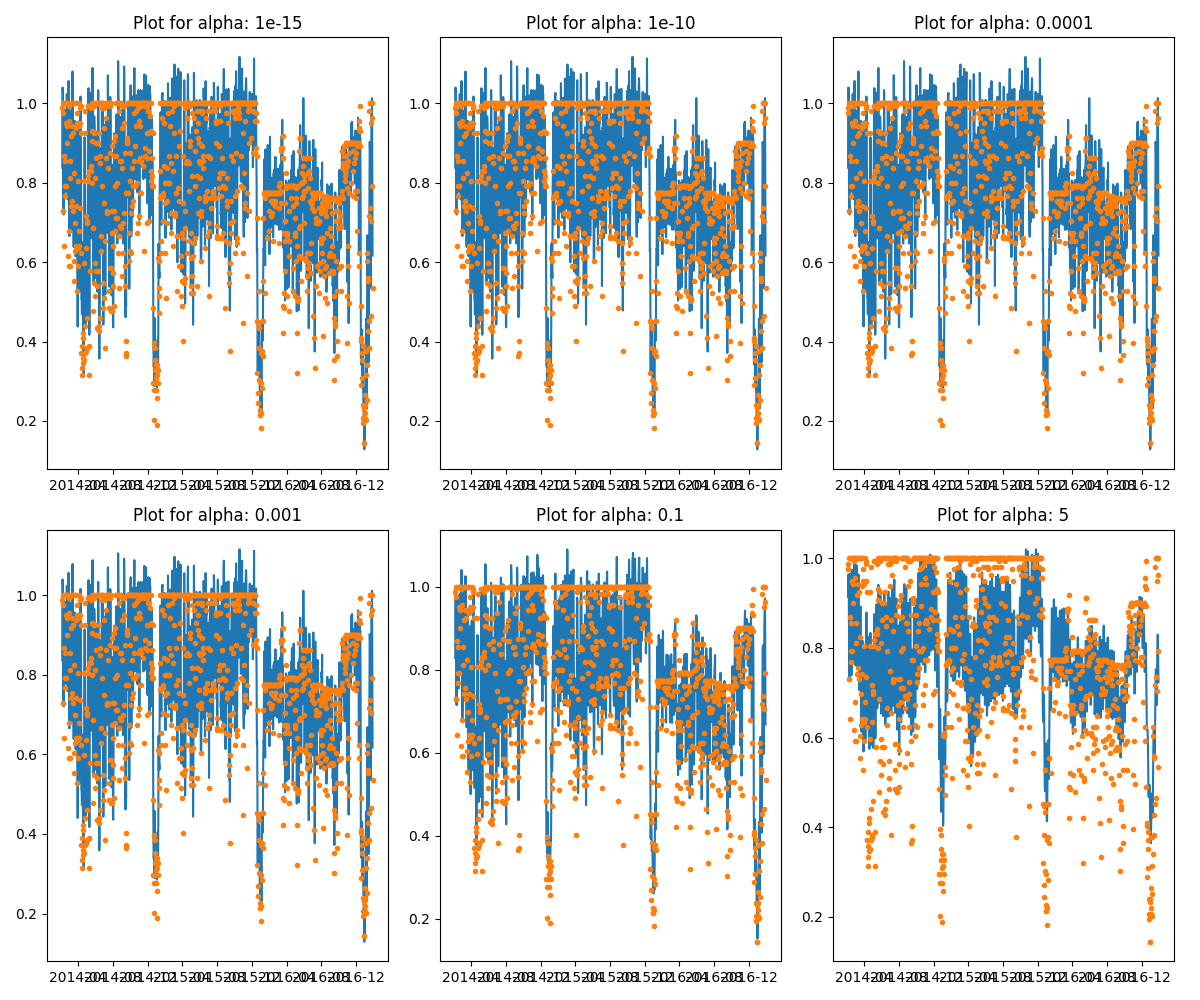
\includegraphics[width=\maxwidth,height=10cm]{figures/alphas_ridge.png}  
  \caption{Efecto de $\alpha$ sobre las predicciones generadas}
\end{figure}

Como podemos observar, a mayor valor de $\alpha$ disminuye la varianza de las predicciones pero incrementa el sesgo. A menor valor de $\alpha$ tenemos un comportamiento opuesto.

La regresión de \emph{Ridge} nos regresa una matriz de coeficientes que multiplican a las variables de entrada del modelo, de tal forma que $y=\beta_0 + \beta_1*x_1 + \beta_2*x_2 + ,..., \beta_n*x_n$. Para generar predicciones para días futuros lo que el modelo internamente hace es tomar la matriz de coeficientes generados por la regresión y los multiplica por la matriz de predictores y como resultado arroja la $\hat{y}$.

El \emph{MAPE} obtenido para este modelo con el conjunto de datos de validación, utilizando una ventana de rezagos de 400 días  para pronósticar una ocupación futura y $\alpha = 1*e^{-15}$ fue de 15.1815\%.

\subsection*{Modelo de análisis de series temporales SARIMA}

Como se mencionó en el capítulo anterior, para poder encontrar el modelo con mejor desempeño se implementó un algorítmo de \emph{grid search}. Dicho algorítmo toma todos los valores definidos para los hiperparámetros del modelo y lo ajusta sobre los datos de entrenamiento. Lo que este algorítmo busca es el conjunto de valores para los hiperparámetros que logran un mejor desempeño del modelo.

En este caso el modelo \emph{SARIMA} con mejor desempeño fue el \emph{SARIMA(1, 0, 0)x(1, 0, 1, 7)} con un \emph{AIC=-3051.784}.

A continuación se presentan las gráficas de diagnóstico obtenidas para dicho modelo. Lo que se busca en estas gráficas es que los residuales no esten correlacionados y se distribuyan normalmente con media = 0. En caso de no tener estos resultados se debe considerar mejorar el modelo ya que podemos incurrir en un alto riesgo de \emph{falsos positivos} en nuestros coeficientes.

\begin{figure}[H]
  \centering
      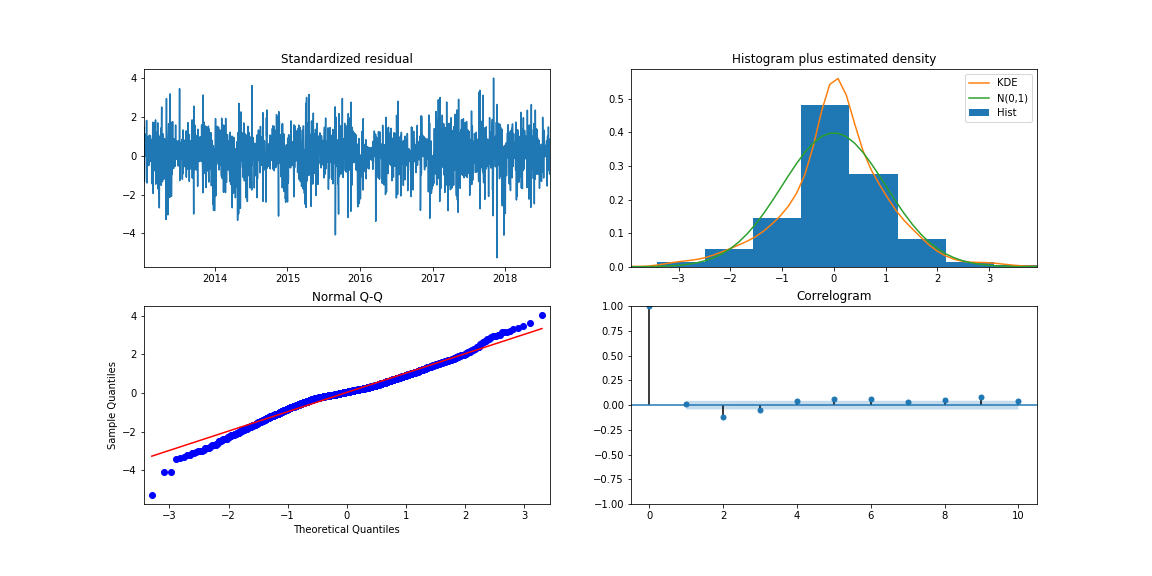
\includegraphics[width=\maxwidth,height=10cm]{figures/sarimax_summary.png}  
  \caption{Diagnóstico del modelo SARIMA(1, 0, 0)x(1, 0, 1, 7)}
\end{figure}


Observando la gráfica presentada podemos confiar en los resultados obtenidos ya que los residuales obtenidos no estan correlacionados y se distribuyen normalmente con media = 0. Esto lo podemos observar poniendo atención en los siguientes puntos:

\begin{itemize}
  \item La gráfica \emph{QQ} se ajusta linealmente a lo largo de la muestra con distribución normal, es decir, todos los puntos caen sobre la línea roja.
  \item La gráfica \emph{KDE} muestra que los residuales son consistentes con una distribución normal con media = 0.
  \item El correlograma muestra una baja autocorrelación para los residuales cuando los rezagos son mayores a 0.
\end{itemize}

Podemos confirmar el desempeño del modelo con el valor del \emph{MAPE} obtenido con el conjunto de datos de validación de 14.8880\% el cual demostró ser el mejor modelo de los tres propuestos.

\subsection*{Comparación de desempeño de modelos de predicción de demanda}

En la siguiente tabla se muestran el desempeño de cada uno de los modelos utilzando el \emph{MAPE} como medida de desempeño:

\begin{table}[H]
\begin{tabular}{lllllllllllll}
Modelo  & MAPE      \\
Regresión Lineal Generalizada con Liga Poisson & 17.67 \\
Regresion de Ridge & 15.1815 \\
SARIMA & 14.8880
\end{tabular}
\caption{Desempeño de modelos propuestos} 
\end{table}

Como se puede observar el modelo que tuvo un mejor desempeño, de acuerdo al \emph{MAPE} fue el modelo de análisis de series temporales \emph{SARIMAX}. Los resultados de este modelo fueron alimentados al modelo de optimización de ingresos.

\subsection*{Modelo de maximización de ingresos}

El modelo de recomendaciones de precio toma como entrada la demanda pronósticada por el módelo de pronóstico de demanda con mejor desempeño de acuerdo al \emph{MAPE}. A partir de ahi, se define un problema de maximización sujeto a restricciones y se arroja una matriz que contiene los precios para un tipo de cuarto dependiendo del inventario disponible dentro de la propidad.

A continuación se muestra un extracto del resultado:

\begin{table}[H]
  \centering
  \csvautotabular{data/rates.csv}\par
  \caption{Matriz de asignacion de precio por inventario disponible}
\end{table}

La manera en la que se debe interpretar esta matriz es la siguiente: Para el día 14 de Agosto de 2018, las habitaciones sencillas de este hotel deben de tener un precio de \$1295.06 MXN si el inventario disponible esta entre 121 y 159 habitaciones disponibles. Si se tienen entre 81 y 120 habitaciones disponibles, el precio debe de ser de \$1490.73 MXN y así sucesivamente. De esta manera podemos asignar un lote de habitaciones a diferentes rangos de precios siendo las últimas habitaciones disponibles las que tengan el precio más alto.


A continuación se presenta una gráfica con los resultados obtenidos por el modelo de maximización de ingresos:

\begin{figure}[H]
  \centering
      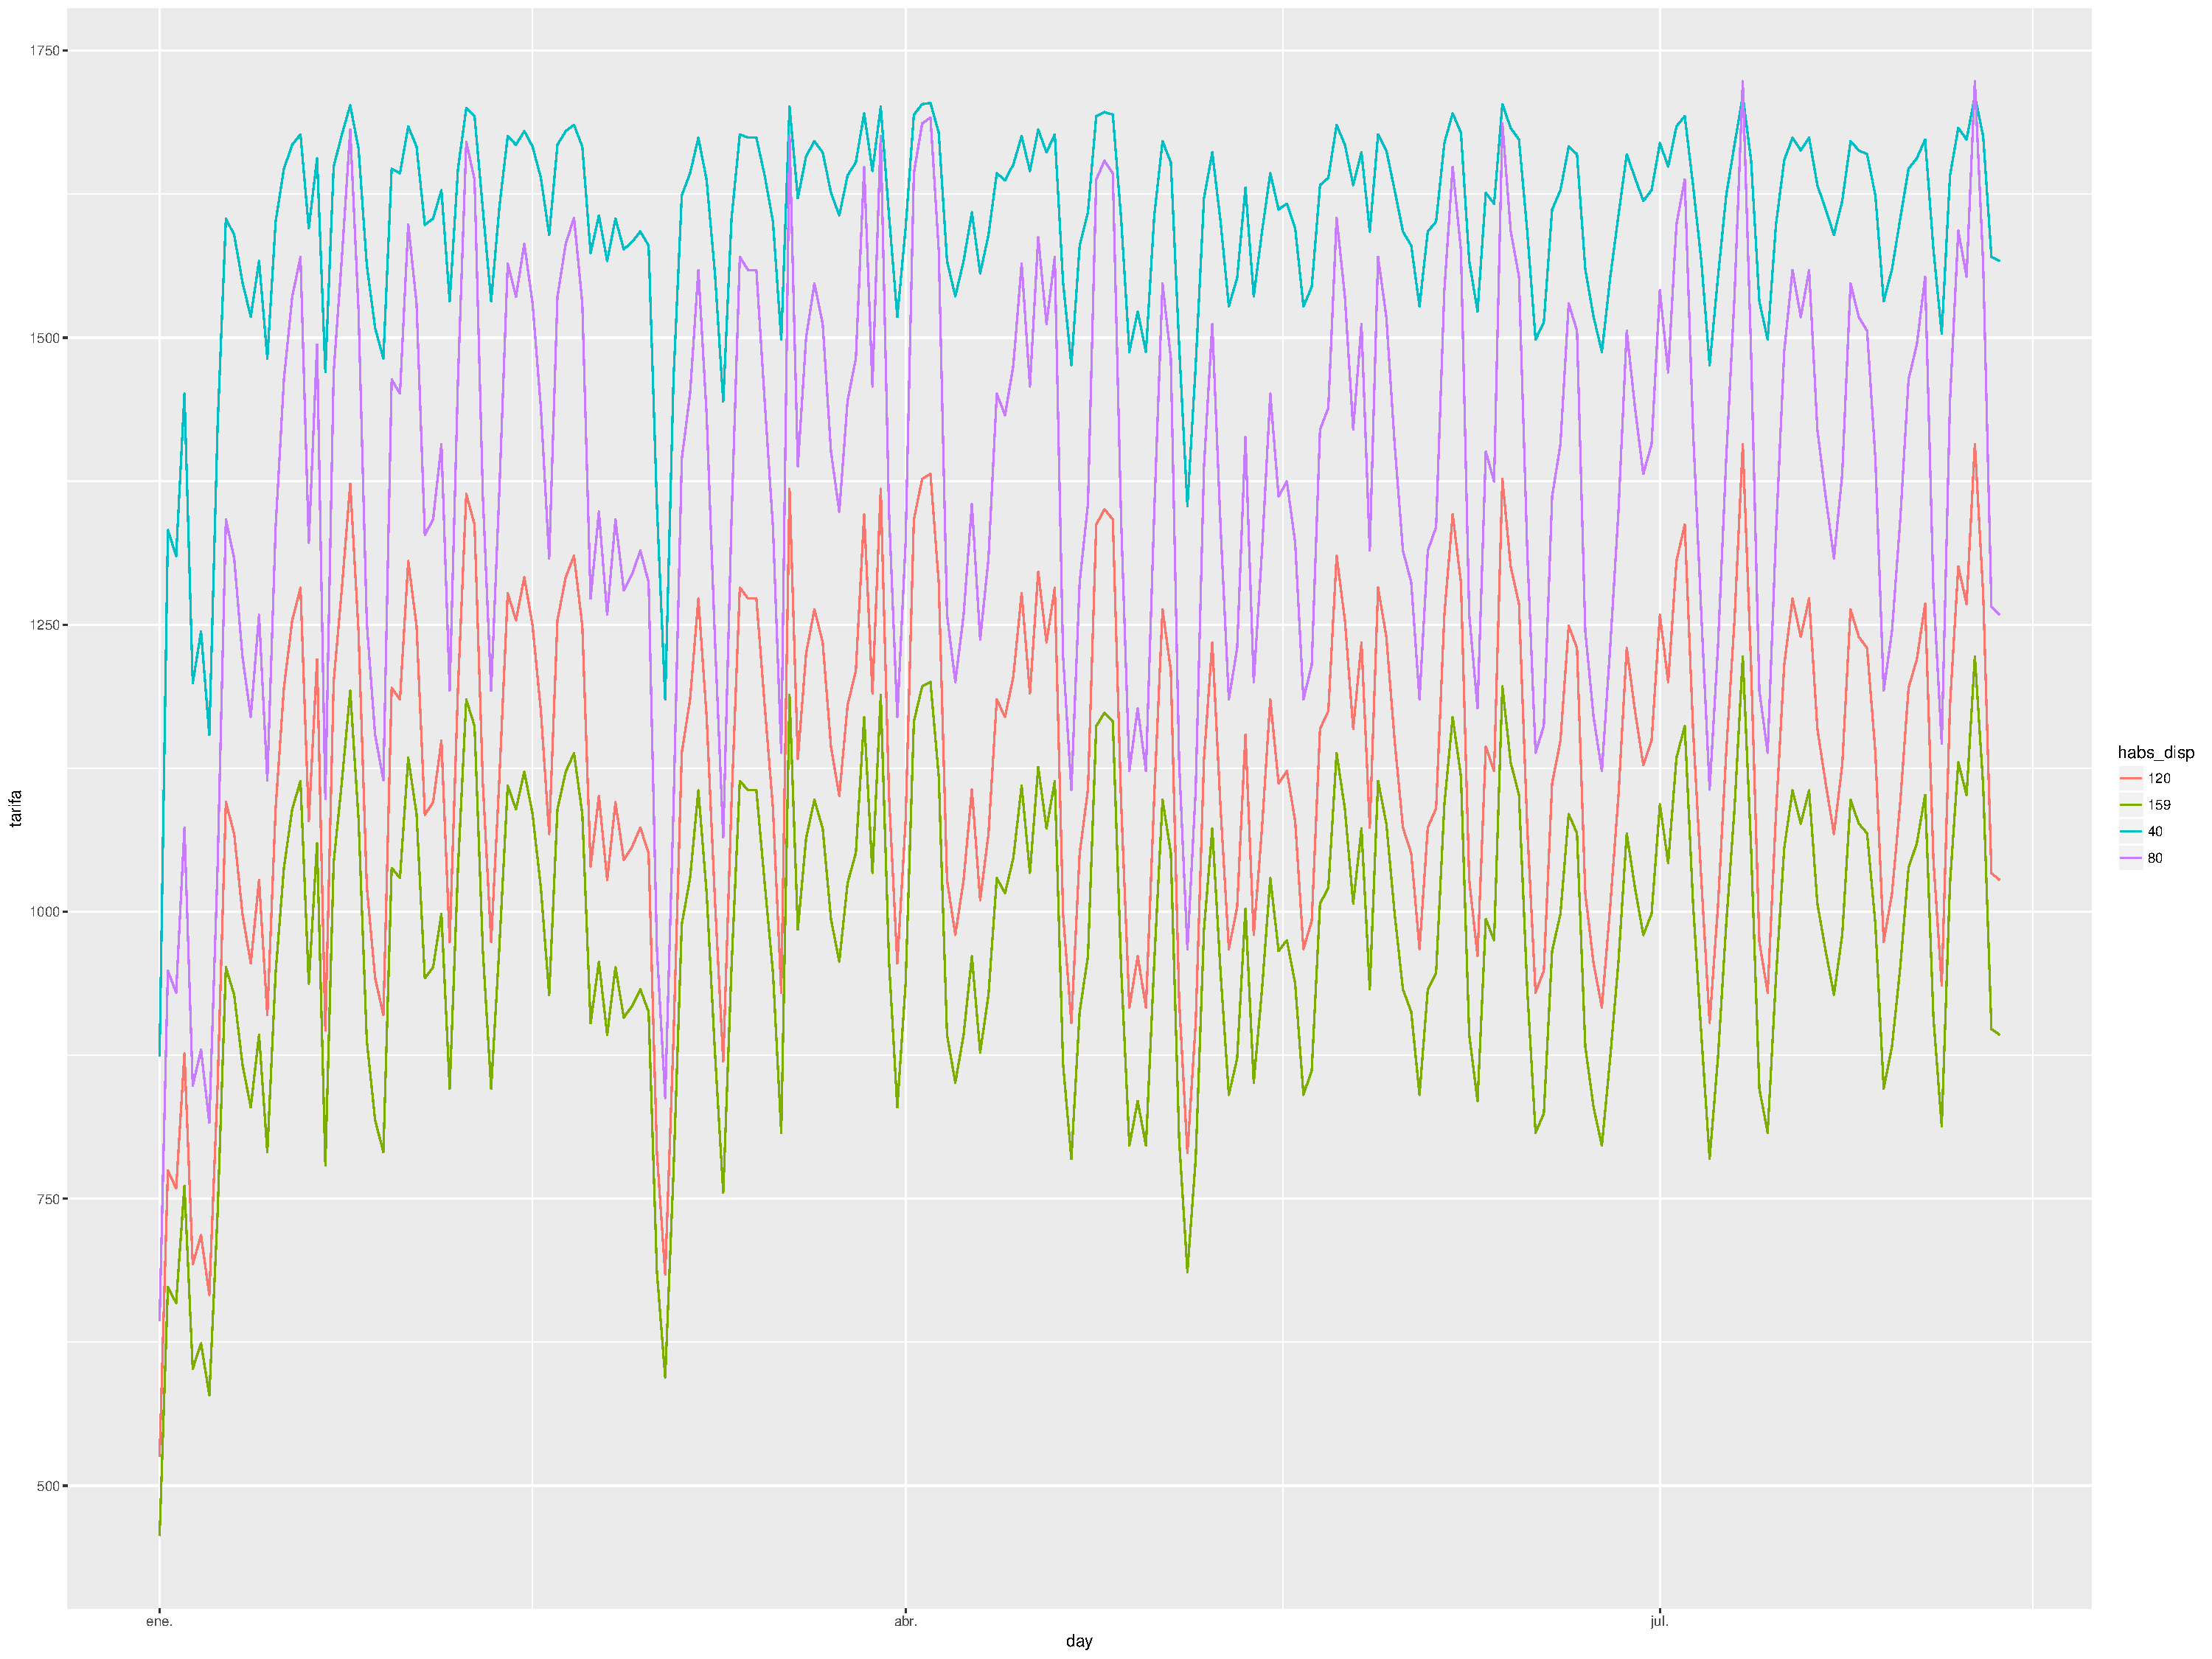
\includegraphics[width=\maxwidth,height=10cm]{figures/Pricing_graph-1}  
  \caption{Precios propuestos para distintos niveles de inventario disponible}
\end{figure}


Para medir el desempeño del modelo de maximización de ingresos, se tomaron los resultados y se calcularon las tarifas promedio a partir de los datos obtenidos y se compararon contra las tarifas promedio reportadas por la propiedad para el año 2018.

\begin{figure}[H]
  \centering
      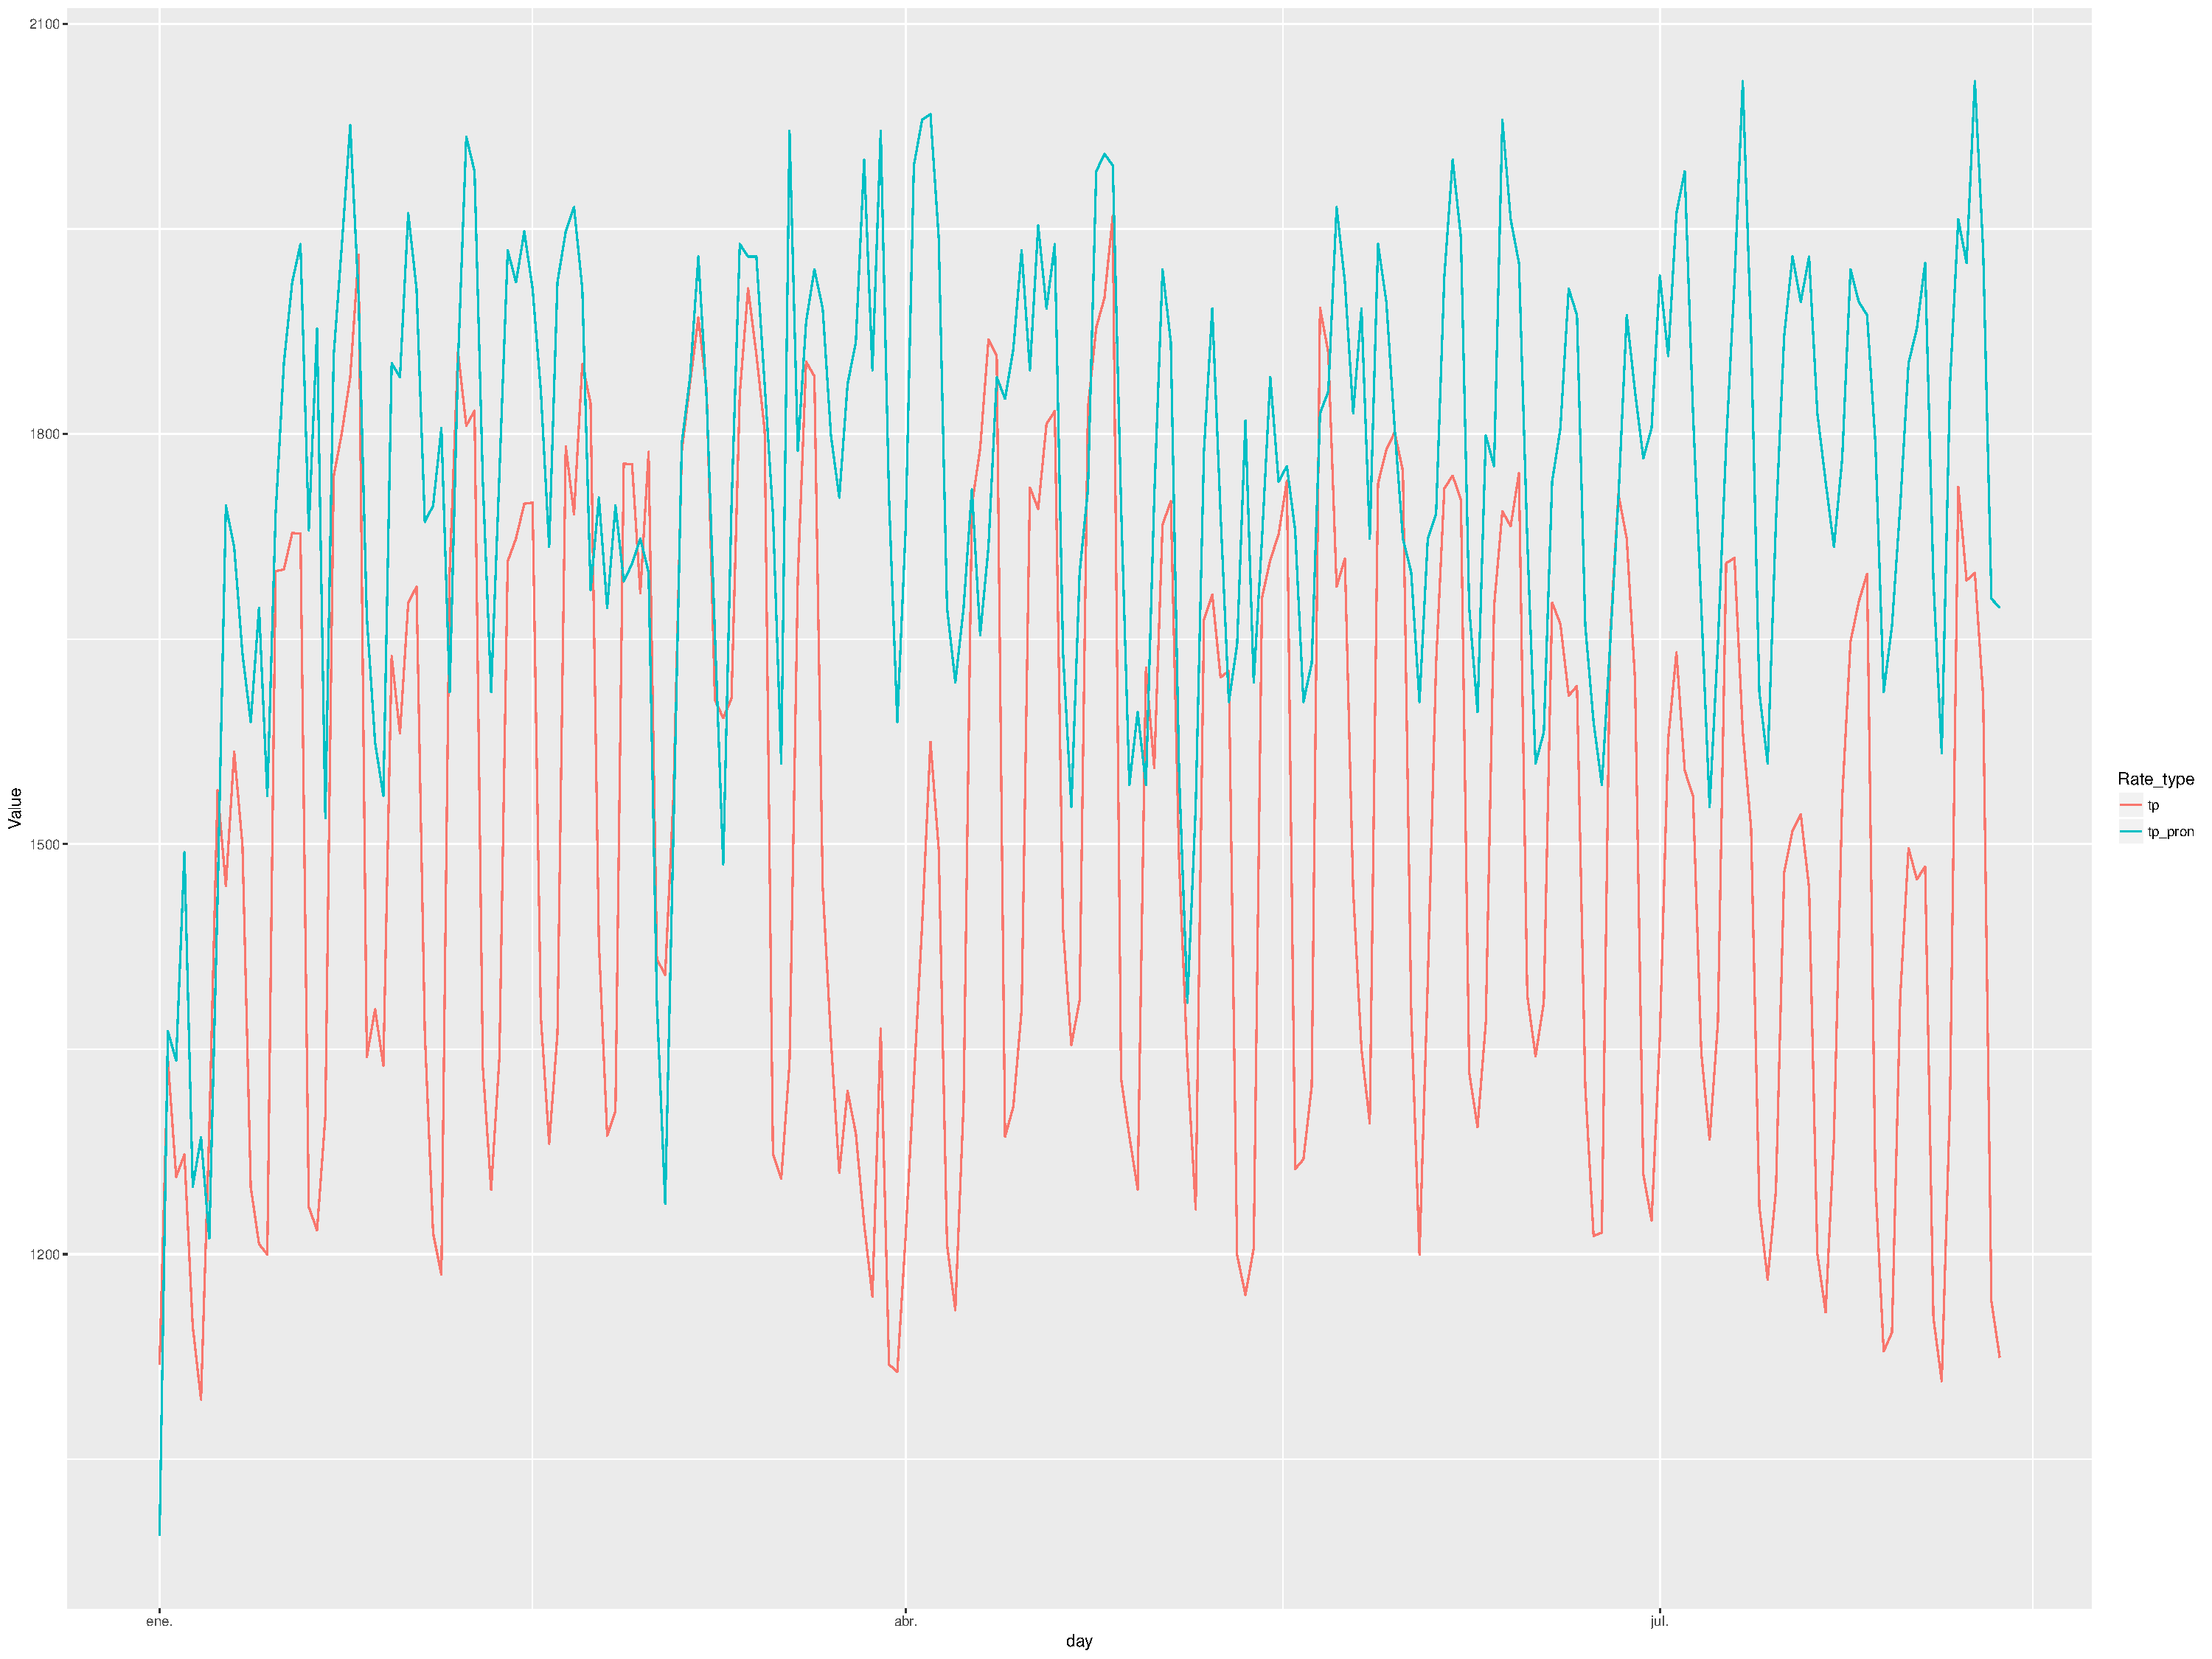
\includegraphics[width=\maxwidth,height=10cm]{figures/Pricing-1}  
  \caption{Tarifa Promedio optimizada vs Tarifa Promedio Real}
\end{figure}


Si obtenemos la diferencia de tarifas promedio, notamos que si se utilizara el resultado del modelo de optimización tendríamos un aumento en los ingresos de aproximadamente 5947.626 MXN para el periodo del 14 de agosto 2018 al 9 de septiembre del 2019. Sin embargo, para poder validar este resultado se propone implementar este modelo dentro de la propiedad y comprobar sus resultados en la operación.




